\documentclass[11pt,a4paper]{article}

\usepackage[utf8]{inputenc}
\usepackage[T1]{fontenc}
\usepackage{lmodern}
\usepackage{microtype}
\emergencystretch=3em
\usepackage[margin=2.6cm]{geometry}
\usepackage{amsmath,amssymb,amsthm,mathtools}
\usepackage{booktabs,array,longtable}
\usepackage{enumitem}
\usepackage{tikz}
\usetikzlibrary{arrows.meta,positioning}
\usepackage[colorlinks=true,linkcolor=blue!50!black,citecolor=blue!50!black,urlcolor=blue!50!black]{hyperref}
\usepackage{thmtools}
\usepackage[capitalise,noabbrev]{cleveref}

\declaretheorem[name=Theorem,numberwithin=section]{theorem}
\declaretheorem[name=Lemma,sibling=theorem]{lemma}
\declaretheorem[name=Proposition,sibling=theorem]{proposition}
\declaretheorem[name=Corollary,sibling=theorem]{corollary}
\declaretheorem[name=Definition,sibling=theorem,style=definition]{definition}
\declaretheorem[name=Example,sibling=theorem,style=definition]{example}
\declaretheorem[name=Assumption,sibling=theorem,style=definition]{assumption}
\declaretheorem[name=Remark,sibling=theorem,style=remark]{remark}

\newcommand{\J}{\mathcal{J}}
\newcommand{\M}{\mathcal{M}}
\newcommand{\U}{\mathcal{U}}
\newcommand{\Sites}{\mathcal{S}}
\newcommand{\K}{\mathcal{K}}
\newcommand{\Res}{\mathcal{R}}
\newcommand{\Z}{\mathbb{Z}}
\newcommand{\R}{\mathbb{R}}
\newcommand{\code}[1]{\texttt{#1}}
\newcommand{\pin}{\mathrm{in}}
\newcommand{\pout}{\mathrm{out}}
\newcommand{\bill}{\mathrm{bill}}
\newcommand{\occ}{\mathrm{occ}}
\newcommand{\run}{\mathrm{run}}
\newcommand{\status}[1]{\textsf{\small[#1]}}

\title{The FED-HPC arc-flow model with multi-node jobs,\\
GPU nodes and geo-distributed I/O}
\author{fedhpc project notes}
\date{23 November 2026}

\begin{document}
\maketitle

\begin{abstract}
This note brings together in one model three extensions of the FED-HPC
space-time (arc-flow) MILP that are spread over the code, the CCGrid
paper draft and the design notes: (i) \emph{multi-node} jobs that hold $q_j>1$
instances of one type at the same time, (ii) \emph{GPU} requirements, and
(iii) \emph{geo-distributed I/O}, where each job has a data origin and a result
destination and the transfer time and price depend on the (job, type) pair.
Extensions (i) and (ii) are implemented in \code{Instance.build}
(\code{src/fedhpc/data.py}) and \code{SpaceTimeFormulation}
(\code{src/fedhpc/formulations.py}) since commit \code{0f0e42d}. Extension
(iii) is the ``Level~1'' design of \code{docs/geo\_distributed\_transfer.md},
implemented on branch \code{geo-distributed-io} (commit \code{6c73896}, not yet
on \code{main}, whose code has only the special case of one home site and
output only). We state the data, the derived parameters,
the network, the full model and its objectives. We prove that the multi-unit
flow rows enforce capacity exactly, and for each exact reduction (R1, R2, R3,
LX, N1, N2) we check whether it survives the extensions.
\Cref{sec:diff} lists, item by item, what changes relative to the
formulation of the CCGrid draft.
\end{abstract}

\tableofcontents

%======================================================================
\section{Scope and status}\label{sec:scope}
%======================================================================

Time is discrete. A \emph{slot} $u\in\{0,\dots,H-1\}$ is the interval $[u,u+1)$
and a \emph{node} $v\in\{0,\dots,H\}$ is an instant. All durations below are in
slots; converting from physical units (division by the slot length $\Delta$) is
done before the model is built. Every statement is tagged with its status:
\status{impl} means implemented and tested on \code{main}, \status{branch}
means implemented and tested on branch \code{geo-distributed-io} only,
\status{proposed} means specified here but not in the code, and
\status{paper} means proved here and not machine-checked.

\begin{center}
\small
\begin{tabular}{@{}lll@{}}
\toprule
Extension & Status & Where \\
\midrule
Multi-node jobs ($q_j\ge1$), multi-unit running jobs & \status{impl} &
  \code{Job.nodes}, \code{RunningJob.units} \\
GPU per instance ($q^{\mathrm{gpu}}_j$, $C^{\mathrm{gpu}}_m$) & \status{impl} &
  \code{Job.gpu}, \code{InstanceType.gpu} \\
Output egress to one home site, cloud only & \status{impl} &
  \code{io\_volume}, \code{io\_time}, \code{cost\_io} \\
Sites, origin/dest., input staging, links, allowed sites & \status{branch} &
  \cref{sec:geo,sec:impl} \\
Geo-I/O \emph{and} multi-node in one instance & \status{branch} &
  \cref{sec:combined} \\
\bottomrule
\end{tabular}
\end{center}

\noindent\sloppy The single-site, single-node, CPU-only model is the one in the
CCGrid draft
(\code{MOFE\_FEDHPC\_CCGRID}, Section~III) and in
\code{docs/formulation\_reductions.tex}. This note reduces to that model when
$q_j=1$, $q^{\mathrm{gpu}}_j=0$ and $|\Sites|=1$ (\cref{rem:reduces}).

%======================================================================
\section{Data}\label{sec:data}
%======================================================================

\subsection{Sites, types and resources}

\begin{itemize}[leftmargin=*]
\item $\Sites$: a finite set of \emph{sites}, i.e.\ geographic locations that
  hold data. Each on-premises cluster is a site, and so is each cloud region.
  \status{branch}
\item $\M$: \emph{instance types}. A type is a pool of homogeneous instances
  (nodes or VMs) at one site $\sigma(m)\in\Sites$. Each type has a capacity
  $N_m\in\Z_{>0}\cup\{\infty\}$ (number of instances; $\infty$ for cloud), a
  performance factor $P_m>0$, a deployment time $\pi_m\ge0$ (it occupies the
  instance but is not billed), and per-instance resource capacities
  $C^r_m\ge0$ for
  \[
    r\in\Res=\{\mathrm{cpu},\mathrm{mem},\mathrm{stor},\mathrm{gpu}\}.
  \]
  The rates are $\kappa^{\mathrm{VM}}_m$ (per instance and slot),
  $\kappa^{\mathrm{S}}_m$ (per unit of storage, instance and slot) and an
  optional one-off usage charge $U_m\ge0$. On-premises types have
  $\kappa^{\mathrm{VM}}_m=\kappa^{\mathrm{S}}_m=U_m=0$.
\item A GPU partition is modelled as its own type with $C^{\mathrm{gpu}}_m>0$.
  A CPU partition has $C^{\mathrm{gpu}}_m=0$. \status{impl}
\end{itemize}

\subsection{Jobs}

Each job $j\in\J$ is released at $a_j$ (it may be negative inside a rolling
window: it has already waited) and has
\begin{itemize}[leftmargin=*]
\item a base execution time $e_j\ge0$ and an integral priority weight
  $w_j\in\Z_{\ge0}$;
\item a \emph{node count} $q_j\in\Z_{\ge1}$: the job runs on $q_j$ instances of
  \emph{one} type, all starting and finishing together (gang scheduling)
  \status{impl};
\item per-instance demands $q^r_j\ge0$, $r\in\Res$, GPUs included
  \status{impl};
\item geo-distributed I/O \status{branch}: an \emph{origin} site $o_j$ that
  holds the job's input data, of volume $\iota^\pin_j\ge0$, and a
  \emph{destination} site $d_j$ that must receive its results, of volume
  $\iota^\pout_j\ge0$. By default $d_j=o_j$, the user's home cluster;
\item a set of \emph{allowed sites} $\Sites_j\subseteq\Sites$ (default
  $\Sites$), e.g.\ for a site-licensed code or an incompatible software stack
  \status{branch}.
\end{itemize}

\subsection{Transfer links}\label{sec:links}

Each directed link $(s,s')$ between two sites \status{branch} has a time
$\theta_{ss'}\ge0$ (slots per GB) and a price $\kappa_{ss'}\ge0$ (\$ per GB),
with $\theta_{ss}=\kappa_{ss}=0$: local data moves at no cost
(\code{Link(src, dst, time, cost)}; a missing non-local link is an error). The
generator \code{geo\_gen.py} sets $\theta=1/B_{\mathrm{eff}}$ with
$B_{\mathrm{eff}}=\min(\text{source read},\text{network},\text{sink write})$
(Liu et al., HPDC'17). Because links are indexed by sites and not by types,
every cloud type of a region shares one rate. Per-VM bandwidth caps would
need a site per VM family. Typical values:
\begin{itemize}[leftmargin=*]
\item cloud to anywhere: $\kappa^\pout>0$ (internet egress price);
\item anywhere to cloud: $\kappa^\pin=0$ (ingress is free);
\item between research-network sites: $\kappa=0$, $\theta>0$.
\end{itemize}

\subsection{Running jobs}

$\K$ is the set of jobs already running at $t=0$. They are fixed and not
re-optimised. Job $k\in\K$ occupies $u_k\in\Z_{\ge1}$ instances of a
finite-capacity type $m_k$ until slot $\bar e_k=\min(e_k,H)$, with $\bar e_k\ge1$.
Define
\[
  n^\run_m=\sum_{k\in\K:m_k=m}u_k\le N_m,
  \qquad
  g_{mv}=\sum_{k\in\K:m_k=m,\ \bar e_k=v}u_k,
  \qquad
  n^\run_m(u)=\sum_{k\in\K:m_k=m,\ u<\bar e_k}u_k .
\]
Here $g_{mv}$ counts the ``ghost completions'' at node $v$, and $n^\run_m(u)$
counts the instances held in slot $u$.

%======================================================================
\section{Derived parameters}\label{sec:derived}
%======================================================================

\subsection{Feasible types}

\begin{equation}\label{eq:F}
  F_j=\bigl\{m\in\M:\ q^r_j\le C^r_m\ \ \forall r\in\Res,\ \ q_j\le N_m,
  \ \ \sigma(m)\in\Sites_j\bigr\}.
\end{equation}
The GPU condition $q^{\mathrm{gpu}}_j\le C^{\mathrm{gpu}}_m$ sends GPU jobs to
GPU types only. The node condition $q_j\le N_m$ removes types too small to
ever hold the job. \status{impl} The site condition restricts the job to its
allowed sites. \status{branch} We require $F_j\neq\emptyset$
(\code{build()} raises otherwise).

\subsection{Transfer time and transfer cost}\label{sec:geo}

For $m\in F_j$ \status{branch} (\code{io\_t}, \code{io\_c} in \code{Instance.build}),
\begin{align}
  \tau_{jm} &= \theta_{o_j\sigma(m)}\,\iota^\pin_j+\theta_{\sigma(m)d_j}\,\iota^\pout_j,
  \label{eq:tau}\\
  \kappa_{jm} &= \kappa_{o_j\sigma(m)}\,\iota^\pin_j+\kappa_{\sigma(m)d_j}\,\iota^\pout_j.
  \label{eq:kappa}
\end{align}
Both are \emph{job-level} quantities and are not multiplied by $q_j$: the data
of a multi-node job is moved once, not once per instance. This is how the
current code treats $\iota_j$ (\code{cost\_io * io\_volume} in
\code{Instance.build}).

\paragraph{The case implemented today.} One home site $h$; $\iota^\pin_j=0$;
$d_j=h$ for every job; $\iota^\pout_j=\iota_j$;
per-type rates $\tau^{\mathrm{IO}}_m$ and $\kappa^{\mathrm{IO}}_m$ in place of
the links, both zero on on-prem types (\code{instance\_gen.py}). Then
$\tau_{jm}=\tau^{\mathrm{IO}}_m\iota_j$ and
$\kappa_{jm}=\kappa^{\mathrm{IO}}_m\iota_j$. \status{impl} On the branch this
\emph{per-type mode} stays the default and is bit-identical to \code{main}. A
non-empty \code{links} switches to the site-aware mode, which requires
$\tau^{\mathrm{IO}}_m=\kappa^{\mathrm{IO}}_m=0$ so that no transfer is priced twice.

\subsection{Durations, costs and start sets}

\begin{align}
  p^\bill_{jm} &= e_j/P_m+\tau_{jm},
  \label{eq:pbill}\\
  p_{jm} := p^\occ_{jm} &= \max\bigl\{1,\ \lceil p^\bill_{jm}+\pi_m\rceil\bigr\}\in\Z_{\ge1},
  \label{eq:pocc}\\
  c_{jm} &= \delta\cdot\operatorname{round}\!\Bigl(
     \bigl[\kappa_{jm}
     + q_j\,(\kappa^{\mathrm{VM}}_m+\kappa^{\mathrm{S}}_m q^{\mathrm{stor}}_j)\,p^\bill_{jm}\bigr]/\delta\Bigr),
  \label{eq:cost}\\
  T_{jm} &= \bigl\{t\in\Z:\ \max(0,\lceil a_j\rceil)\le t\le H-p_{jm}\bigr\}.
  \label{eq:T}
\end{align}
Here $\delta>0$ is the cost resolution (\code{cost\_resolution}). VM time and
storage are billed for each of the $q_j$ instances, and the transfer once.
The transfer time is part of $p^\bill$ and therefore also of $p$: all $q_j$
instances stay held (and, in the cloud, billed) while data is staged in and
out (see \cref{rem:staging}).

\begin{remark}[Billing granularity]
The CCGrid draft rounds $p^\bill$ up to whole slots before pricing (billing in
blocks of $\Delta$). The code prices the continuous $p^\bill$ and rounds the
cost to the grid $\delta$. Formula \eqref{eq:cost} follows the code. The
model does not depend on which rule is used, provided $c_{jm}$ does not depend
on the start time.
\end{remark}

\begin{example}[One job, three types]\label{ex:one}
A job with $q_j=2$, $q^{\mathrm{gpu}}_j=1$, $e_j=8$, input
$\iota^\pin_j=50$\,GB and output $\iota^\pout_j=20$\,GB, with $o_j=d_j=A$.
The types are
$m_A$ (site $A$, $P=1$, $N=4$), $m_B$ (site $B$, $P=2$, $N=2$, research
link $\theta_{AB}=\theta_{BA}=0.02$ slot/GB, $\kappa=0$) and a cloud type $m_c$ at
site $C$ ($P=2$, $N=\infty$, $\pi=1$, $\theta_{AC}=0.01$, $\theta_{CA}=0.02$,
$\kappa_{AC}=0$, $\kappa_{CA}=0.09$\,\$/GB, $\kappa^{\mathrm{VM}}=3$\,\$/slot,
$\kappa^{\mathrm{S}}=0$). All three are GPU types.

\begin{center}
\begin{tabular}{@{}lccccc@{}}
\toprule
type & $e_j/P_m$ & $\tau_{jm}$ & $p^\bill_{jm}$ & $p_{jm}$ & $c_{jm}$ \\
\midrule
$m_A$ & 8 & 0 & 8 & 8 & 0 \\
$m_B$ & 4 & $1.0+0.4$ & 5.4 & 6 & 0 \\
$m_c$ & 4 & $0.5+0.4$ & 4.9 & 6 & $1.8+2\cdot3\cdot4.9=31.2$ \\
\bottomrule
\end{tabular}
\end{center}
The remote research cluster $B$ finishes as early as the cloud at no cost, even
after staging. In the model of the current code, $B$ would show $p=4$, because
on-prem transfer is free and instantaneous there. On every type the job's arc
carries 2 units of flow.
\end{example}

%======================================================================
\section{The arc-flow network}\label{sec:network}
%======================================================================

For each type $m$ with finite capacity, $G_m$ is a DAG on the nodes
$\{0,\dots,H\}$ with
\begin{align*}
  A^{\mathrm{wait}}_m&=\{(v,v+1):0\le v<H\},\\
  A^{\mathrm{proc}}_m&=\{(j,t,t+p_{jm}):\ m\in F_j,\ t\in T_{jm}\}.
\end{align*}
A wait arc carries the instances that are idle in slot $v$. The processing arc
$(j,t,t+p_{jm})$ carries \emph{$q_j$ units} of flow when selected: the $q_j$
instances leave the idle pool together at $t$ and return together at
$t+p_{jm}$. $N_m-n^\run_m$ units enter at node $0$, the running jobs inject
$g_{mv}$ units at node $v$, and $N_m$ units leave at node $H$. For an unbounded
type the code sets $N_m:=\sum_j q_j$, which can never bind.

\begin{figure}[h]
\centering
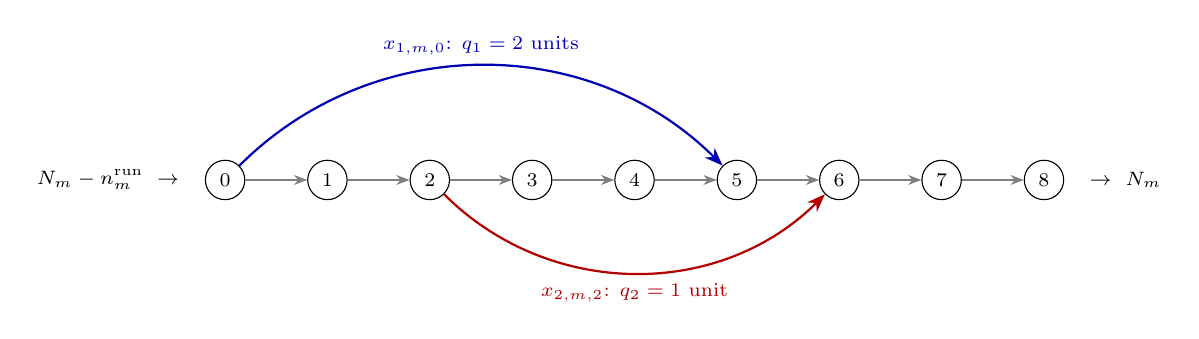
\begin{tikzpicture}[>=Stealth,node distance=1.25cm,
  t/.style={circle,draw,inner sep=1.5pt,minimum size=5mm,font=\scriptsize}]
  \foreach \i in {0,...,8} { \node[t] (n\i) at (1.3*\i,0) {\i}; }
  \foreach \i [evaluate=\i as \j using int(\i+1)] in {0,...,7}
    { \draw[->,gray] (n\i) -- (n\j); }
  \draw[->,thick,blue!70!black] (n0) to[bend left=45]
     node[above,font=\scriptsize]{$x_{1,m,0}$: $q_1=2$ units} (n5);
  \draw[->,thick,red!70!black] (n2) to[bend right=45]
     node[below,font=\scriptsize]{$x_{2,m,2}$: $q_2=1$ unit} (n6);
  \node[font=\scriptsize,left=0.2cm of n0] {$N_m-n^\run_m\ \to$};
  \node[font=\scriptsize,right=0.2cm of n8] {$\to\ N_m$};
\end{tikzpicture}
\caption{The network $G_m$ for one type. Gray: wait arcs ($y_{mv}$). Colored:
processing arcs. A multi-node arc carries $q_j$ units.}
\end{figure}

%======================================================================
\section{The model}\label{sec:model}
%======================================================================

Let $\M^{\mathrm{flow}}\subseteq\M$ be the types that keep a flow network
(after R1, \cref{sec:reductions}, the bounded ones; without reductions, all).
The variables are $x_{jmt}\in\{0,1\}$ (job $j$ starts on $m$ at $t$),
$y_{mv}\ge0$ (instances of $m$ idle in slot $v$) and $z_m\in\{0,1\}$ for each
type with $U_m>0$.

\begin{align}
  &\sum_{m\in F_j}\sum_{t\in T_{jm}}x_{jmt}=1
    && j\in\J, \label{eq:assign}\\[2pt]
  &y_{m,v-1}+\!\!\sum_{\substack{j:\,m\in F_j\\ v-p_{jm}\in T_{jm}}}\!\! q_j\,x_{jm,v-p_{jm}}+g_{mv}
   = y_{mv}+\!\!\sum_{\substack{j:\,m\in F_j\\ v\in T_{jm}}}\!\! q_j\,x_{jmv}
    && m\in\M^{\mathrm{flow}},\ v\in\{0,\dots,H\}, \label{eq:flow}\\[2pt]
  &\textstyle y_{m,-1}:=N_m-n^\run_m,\qquad y_{mH}:=N_m
    && m\in\M^{\mathrm{flow}}, \label{eq:boundary}\\[2pt]
  &\sum_{t\in T_{jm}}x_{jmt}\le z_m
    && j\in\J,\ m\in F_j,\ U_m>0, \label{eq:fixed}\\[2pt]
  &x_{jmt}\in\{0,1\},\quad y_{mv}\in\R_{\ge0},\quad z_m\in\{0,1\}. \label{eq:domains}
\end{align}

Row \eqref{eq:assign} schedules every job exactly once on one type and at one
start. Row \eqref{eq:flow} conserves the instances of type $m$ at node $v$:
idle instances arriving, plus instances released by finishing new and running
jobs, equal idle instances leaving plus instances taken by jobs starting at $v$.
The only difference from the single-node model is the coefficient $q_j$
(\code{units\_at} / \code{flow\_sum} in \code{SpaceTimeFormulation.build}).
GPUs and sites do not appear in the rows. They act only through $F_j$, $p_{jm}$
and $c_{jm}$.

\subsection{Objectives}

\begin{align}
  f_1(x)&=\sum_{j,m,t}w_j\,(t+p_{jm}-a_j)\,x_{jmt}
    &&\text{weighted turnaround,}\label{eq:f1}\\
  f_2(x,z)&=\sum_{j,m,t}c_{jm}\,x_{jmt}+\sum_{m:U_m>0}U_m z_m
    &&\text{monetary cost.}\label{eq:f2}
\end{align}
The lexicographic extreme $(f_1^{\mathrm{lex}},f_2^{\mathrm{lex}})$, the
normalisation and the $\lambda$-scalarisation are those of the CCGrid draft
(Section~III-D) and \code{pareto.py}. Only the reference point needs a change:

\begin{remark}[The zero-cost reference point under geo-I/O]\label{rem:f20}
The draft assumes that a schedule with $f_2=0$ exists, so that
$f_1^0=\min\{f_1:f_2=0\}$. With on-prem links that charge
($\kappa^\pin_{sm}>0$ or $\kappa^\pout_{ms}>0$ between two on-prem sites), or
with a job that fits only cloud types, this can fail. The general form is
$f_2^{\min}=\min f_2$ and $f_1^0=\min\{f_1:f_2=f_2^{\min}\}$. It reduces to the
draft's when $f_2^{\min}=0$. The heuristics already take an \code{f2\_0}
argument.
\end{remark}

%======================================================================
\section{Correctness of the multi-unit flow}\label{sec:correct}
%======================================================================

For a start vector $x$, the \emph{load} of type $m$ in slot $u$ is the number
of instances that new jobs hold in that slot:
\[
  L_{mu}(x)=\sum_{j:\,m\in F_j}\ q_j\!\!\sum_{t\in T_{jm}:\ t\le u<t+p_{jm}}\!\! x_{jmt}.
\]

\begin{proposition}[Flow rows are exact capacity rows]\label{prop:capacity}
\status{paper} Let $x$ satisfy \eqref{eq:assign}. Then a $y$ with
\eqref{eq:flow}--\eqref{eq:boundary} exists if and only if
\begin{equation}\label{eq:cap}
  L_{mu}(x)+n^\run_m(u)\le N_m\qquad\forall m\in\M^{\mathrm{flow}},\ u\in\{0,\dots,H-1\},
\end{equation}
and in that case $y$ is unique and integral:
$y_{mu}=N_m-n^\run_m(u)-L_{mu}(x)$.
\end{proposition}

\begin{proof}
Fix $m$ and $u<H$, and add the rows \eqref{eq:flow} for $v=0,\dots,u$. The $y$
terms telescope to $y_{m,-1}-y_{mu}$. A selected arc $(j,t)$ contributes
$-q_j$ if it starts at or before $u$, and $+q_j$ if it also ends at or before
$u$. Its net contribution is therefore $-q_j$ exactly when $t\le u<t+p_{jm}$,
i.e.\ $-L_{mu}(x)$ in total. The running jobs contribute
$\sum_{v\le u}g_{mv}=n^\run_m-n^\run_m(u)$. With
$y_{m,-1}=N_m-n^\run_m$ the sum gives
\[
  y_{mu}=N_m-n^\run_m(u)-L_{mu}(x).
\]
So $y$ is determined by $x$; it is integral because $q_j$, $N_m$ and $u_k$
are integers, and $y\ge0$ is exactly \eqref{eq:cap}. It remains to check the
row at $v=H$. No arc starts at $H$ ($p_{jm}\ge1$), every arc ends by $H$
(\eqref{eq:T}) and every running job ends by $H$ ($\bar e_k\le H$). Adding all
rows $v=0,\dots,H$ thus gives $y_{m,-1}+n^\run_m=y_{mH}$, i.e.\
$y_{mH}=N_m$, which is \eqref{eq:boundary}. Conversely, if \eqref{eq:cap}
holds, the formula above defines a nonnegative $y$ that satisfies every row.
\end{proof}

\begin{corollary}\status{paper}
The feasible $x$ of \eqref{eq:assign}--\eqref{eq:domains} are exactly the
schedules that place each job once on a type of $F_j$ at a start of $T_{jm}$
and never use more than $N_m$ instances of any type in any slot, running jobs
included. This is the check that \code{Instance.schedule\_violations}
performs. Relaxing $y$ to continuous (\code{continuous\_idle}) loses nothing.
\end{corollary}

\begin{remark}[What gang scheduling means here]
Instances of one type are interchangeable, so the model does not choose
\emph{which} $q_j$ nodes a job gets. Any schedule that satisfies \eqref{eq:cap}
can be given a concrete node assignment. The jobs on a type form an interval
system with load at most $N_m$, and a greedy assignment in start order (an
interval-graph colouring) gives each job $q_j$ distinct nodes. Equivalently,
the integral flow of \eqref{eq:flow} splits into $N_m$ unit paths, $q_j$ of
which traverse arc $(j,t)$. The model ignores network topology and cannot
split one job across types or sites. A job that fits no single type is
infeasible, and the overseer adapter (\code{exclusive\_nodes}) leaves it out.
\end{remark}

\begin{remark}[GPUs are a type attribute, not a pooled resource]
A GPU job gets whole instances of a GPU type, exclusively. Several jobs
sharing the GPUs of one node would need a second capacity dimension per type
(GPUs as well as instances). That would turn \eqref{eq:flow} into a
two-commodity coupling, and it is not modelled. The cost of a GPU is
carried by that type's $\kappa^{\mathrm{VM}}_m$.
\end{remark}

\begin{remark}[Strength of the relaxation]
With $q_j>1$, row \eqref{eq:flow} has the coefficient $q_j$. A fractional
$x_{jmt}=1/q_j$ then uses only one unit of capacity, so the LP bound can be
weaker than in the unit model. The same coefficient is the reason
branch-and-price refuses multi-node instances: a column there is one
instance's path, and $q_j$ paths would have to be synchronised on the same arc.
\end{remark}

\begin{remark}[Staging occupies the nodes]\label{rem:staging}
Folding $\tau_{jm}$ into $p_{jm}$ keeps every proof intact
(\cref{sec:reductions}). It also overstates occupancy, since a real cluster
stages data on transfer nodes while the compute nodes do other work. The
exact alternative is a type-dependent release
$r_{jm}=\lceil a_j+\theta^\pin_{o_jm}\iota^\pin_j\rceil$ and a stage-out tail
$\ell_{jm}=\lceil\theta^\pout_{md_j}\iota^\pout_j\rceil$, with completion
$t+p_{jm}+\ell_{jm}$. That changes $T_{jm}$, $f_1$, \code{bound\_constr}, the
lex rule and R3, and all of them would have to be proved again. The
difference matters only when staging is a sizeable fraction of runtime: about
8\,s/GB makes it relevant only for the ``F'' retention policy.
\end{remark}

\begin{remark}[Reduction to the published model]\label{rem:reduces}
With $q_j=1$, $u_k=1$, $q^{\mathrm{gpu}}_j=C^{\mathrm{gpu}}_m=0$,
$|\Sites|=1$ and $\iota^\pin_j=0$, the model above is the model of the CCGrid
draft and of \code{formulation\_reductions.tex}, symbol for symbol.
\end{remark}

%======================================================================
\section{Exact reductions under the extensions}\label{sec:reductions}
%======================================================================

The proofs in \code{formulation\_reductions.tex} use only these facts:
(a) $f_1$ is nondecreasing in completion times ($w\ge0$); (b) $c_{jm}$ does
not depend on the start time; (c) a type is \emph{unbounded} when its capacity
can never bind, and then a job can always start there at its release; (d) all
data are nonnegative. The extensions change $p_{jm}$ and $c_{jm}$ only
\emph{per (job, type) pair}, and the reductions already read those tables per
pair, so (a), (b) and (d) are unchanged. Fact (c) needs the unit count:
\[
  \U=\Bigl\{m:\ N_m=\infty\ \ \text{or}\ \ N_m-n^\run_m\ge\sum_{j:\,m\in F_j}q_j\Bigr\},
\]
which is \code{unbounded\_types}. Under this definition each job can sit on
$m$ for the whole horizon with its $q_j$ units, so (c) holds.

\begin{center}
\renewcommand{\arraystretch}{1.15}
\begin{longtable}{@{}p{3.1cm}p{1.7cm}p{1.7cm}p{7.0cm}@{}}
\toprule
Reduction & multi-node, GPU & geo-I/O & Why \\
\midrule
\endhead
R1 collapse unbounded & exact & exact & (a)+(b)+(c); no flow network for $m\in\U$. A remote on-prem site can enter $\U$ too. \\
R2 Pareto on unbounded & exact & exact & compares per-job $(C,c)$ pairs only. \\
R3 rejection deadlines & exact & exact & moving $j$ to $k\in\U$ frees $q_j$ units on its old type and never violates \eqref{eq:cap}; the cut uses $p_{jm}$ per pair. \\
LX lex deadlines & exact & exact & $C^*_j=\min_{k\in\U}(\text{release}+p_{jk})$; truncation at $C^*_j-p_{jm}+1$ per pair. \\
N1 normal patterns & exact \status{paper} & exact & \cref{lem:leftshift}; geo-I/O adds distinct $p_{jm}$, which makes the patterns denser. \\
N2 compressed graph & exact \status{paper} & exact & same left-shift argument; loss arcs are unchanged. \\
Integer bound rows & exact & exact & $p_{jm}\in\Z$, $w_j\in\Z$, $c_{jm}\in\delta\Z$. \\
\bottomrule
\end{longtable}
\end{center}

\begin{lemma}[Left shift with multi-unit demand]\label{lem:leftshift}
\status{paper} Take a feasible schedule in which job $j$ starts on a bounded
type $m$ at $t>\max(0,\lceil a_j\rceil)$, and suppose $j$ cannot start at
$t-1$ with all other jobs fixed. Then $t$ is the completion node of some new
or running job on $m$.
\end{lemma}

\begin{proof}
Let $\phi(u)$ be the number of instances of $m$ free in slot $u$ when $j$ is
removed. Moving $j$ from $[t,t+p)$ to $[t-1,t-1+p)$ adds slot $t-1$ and frees
slot $t-1+p$. So the move fails exactly when $\phi(t-1)<q_j$. Feasibility of
the original schedule gives $\phi(t)\ge q_j$, so $\phi(t)>\phi(t-1)$. Between
slots $t-1$ and $t$, $\phi$ decreases only when a job starts at $t$ and
increases only when a job (new or running) completes at $t$. Hence some job
completes at $t$.
\end{proof}

\noindent By induction on starts, every start in a left-shifted schedule is a
release or a completion node. That is the closure property behind N1/N2
(Kramer et al.\ 2020, Algorithm~1, and \code{normal\_pattern\_starts}), which
therefore needs no change for $q_j>1$. The Lean development in
\code{proofs/} covers unit demand only. The multi-unit lemma above is a
paper proof.

%======================================================================
\section{Geo-I/O and multi-node jobs together}\label{sec:combined}
%======================================================================

The two extensions meet only in \eqref{eq:pbill}--\eqref{eq:cost}:
\begin{itemize}[leftmargin=*]
\item the transfer is moved and paid \emph{once per job}. $\tau_{jm}$ and
  $\kappa_{jm}$ do not depend on $q_j$;
\item the staging time is inside $p^\bill_{jm}$, so all $q_j$ instances are
  held for it, and on a cloud type they are also \emph{billed} for it:
  $c_{jm}$ contains $q_j\kappa^{\mathrm{VM}}_m\tau_{jm}$. For a wide job this
  overstates both occupancy and cost (\cref{rem:staging}).
\end{itemize}
No row couples sites with node counts, so \cref{prop:capacity} and
\cref{sec:reductions} hold unchanged on combined instances.

\paragraph{What has been verified.} On branch \code{geo-distributed-io}, the
80 tests of \code{tests/test\_geo.py} and \code{tests/test\_multinode\_gpu.py}
pass (run 2026-11-24). No test on the branch combines the two, and
\code{geo\_gen.py} emits single-node jobs only. A separate check, not
committed, used 24 random instances on the branch code: 3 sites (two on-prem,
one cloud); 6 types, 3 of them GPU types; 10--14 jobs with
$q_j\in\{1,2,3\}$ and GPU demand; and running jobs holding 2 units. On every
instance the reduced SpaceTime, plain SpaceTime, Occupancy and compressed-flow
models gave the same lex-$f_1$ optimum, and the weighted-sum optima at
$\lambda\in\{0.25,0.5,0.75\}$ agreed to $10^{-15}$. Every schedule passed
\code{check\_schedule}, and $c_{jm}=\kappa_{jm}+q_j\kappa^{\mathrm{VM}}_mp^\bill_{jm}$
held on every pair. Multi-node jobs were placed at a remote on-prem site in
3 of the instances.

%======================================================================
\section{Changes relative to the CCGrid draft}\label{sec:diff}
%======================================================================

The draft (\code{MOFE\_FEDHPC\_CCGRID}, Section~III, unchanged on
\code{ccgrid-paper-fixes} and in the working tree as of 2026-11-24) is the
single-node, CPU-only model with per-type output egress. Moving to the model
of this note requires the changes below. \textbf{No variable and no row is
added.} Every change is in the data, in the derived parameters, or in a
coefficient.

\begin{center}
\renewcommand{\arraystretch}{1.15}
\begin{longtable}{@{}p{0.8cm}p{3.0cm}p{4.6cm}p{5.3cm}@{}}
\toprule
\# & Draft & Becomes & Why \\
\midrule
\endhead
D1 & $M$ types, ``non geographically distributed'' & add sites $\Sites$, $\sigma(m)$, links $(\theta_{ss'},\kappa_{ss'})$ & geo-I/O \\
D2 & job: $a_j,e_j,\iota_j,w_j,q^r_j$ & add $q_j$, $q^{\mathrm{gpu}}_j$, $o_j$, $d_j$, $\iota^\pin_j$, $\Sites_j$; $\iota_j\to\iota^\pout_j$ & both \\
D3 & ``each occupies one entire instance'' & occupies $q_j$ entire instances of one type, starting and ending together & multi-node \\
D4 & $R=\{\mathrm{cpu},\mathrm{mem},\mathrm{stor}\}$ & $\Res=R\cup\{\mathrm{gpu}\}$ & GPU \\
D5 & $\tau^{\mathrm{IO}}_m$, $\kappa^{\mathrm{IO}}_m$ per type; zero on-prem & removed; replaced by the links. On-prem links may cost & geo-I/O \\
D6 & $F_j=\{m:q^r_j\le C^r_m\}$ & \eqref{eq:F}: add $q_j\le N_m$ and $\sigma(m)\in\Sites_j$ & both \\
D7 & $p^\bill=e_j/P_m+\tau^{\mathrm{IO}}_m\iota_j$ & $e_j/P_m+\tau_{jm}$, \eqref{eq:tau} & geo-I/O \\
D8 & $c=\kappa^{\mathrm{IO}}_m\iota_j+(\kappa^{\mathrm{VM}}_m+\kappa^{\mathrm{S}}_mq^{\mathrm{stor}}_j)p^\bill\Delta$ & $\kappa_{jm}+q_j(\kappa^{\mathrm{VM}}_m+\kappa^{\mathrm{S}}_mq^{\mathrm{stor}}_j)p^\bill$, \eqref{eq:cost} & both \\
D9 & a processing arc carries 1 unit & carries $q_j$ units & multi-node \\
D10 & flow row with $x_{jmt}$ & coefficient $q_j$ on both sides, \eqref{eq:flow} & multi-node \\
D11 & $N_m\in\Z_{>0}$ for every type & for cloud any $N_m\ge\sum_{j:m\in F_j}q_j$ (code: $\sum_jq_j$) & multi-node \\
D12 & capacity via ``$N_m$ unit paths'' & per-slot load identity, \cref{prop:capacity} & multi-node \\
D13 & $\widehat f_2=f_2/f_2^{\mathrm{lex}}$, $f_1^0$ at $f_2=0$ & $\widehat f_2=(f_2-f_2^0)/(f_2^{\mathrm{lex}}-f_2^0)$, $f_2^0=\min f_2$, $f_1^0$ at $f_2=f_2^0$ (\cref{rem:f20}; already in \code{pareto.py}) & geo-I/O \\
\bottomrule
\end{longtable}
\end{center}

\noindent $f_1$, $f_2$, the assignment row, $T_{jm}$, the variable domains and
the lexicographic and weighted-sum problems keep their form. They are written
in terms of $p_{jm}$ and $c_{jm}$, and only those change.

\paragraph{Draft--code differences that predate the extensions.} These are
worth fixing in the same revision so that the paper matches the code:
\begin{enumerate}[label=(\alph*),leftmargin=*]
\item \emph{Rounding.} The draft sets $p^\bill=\max\{1,\lceil p^{\bill,\mathrm{raw}}/\Delta\rceil\}$
  and $p^\occ=p^\bill+\pi_m$. The code prices the continuous $p^\bill$, rounds
  the cost to $\delta$, and sets $p=\max\{1,\lceil p^\bill+\pi_m\rceil\}$.
\item \emph{Running jobs.} The draft has $y_{m,-1}=N_m$ and no running jobs.
  The code has $y_{m,-1}=N_m-n^\run_m$ and ghost completions $g_{mv}$. Both
  are needed in the rolling-horizon (overseer) setting.
\item \emph{Fixed usage cost} $U_mz_m$ with row \eqref{eq:fixed} is in the
  code but not in the draft. It is needed only if a type has $U_m>0$.
\item \emph{Release in a window.} The code uses
  $T_{jm}\ni t\ge\max(0,\lceil a_j\rceil)$ and keeps a possibly negative $a_j$
  in $f_1$.
\end{enumerate}

%======================================================================
\section{Implementation map}\label{sec:impl}
%======================================================================

\begin{center}
\renewcommand{\arraystretch}{1.1}
\begin{longtable}{@{}p{3.4cm}p{6.2cm}p{3.6cm}@{}}
\toprule
Symbol & Code & Status \\
\midrule
\endhead
$q_j$, $u_k$ & \code{Job.nodes}, \code{RunningJob.units} & \status{impl} \\
$q^r_j$, $C^r_m$, $r\in\Res$ & \code{Job.cpu/mem/stor/gpu}, \code{InstanceType.cpu/mem/stor/gpu} & \status{impl} \\
$F_j$ & \code{Instance.F} & \status{impl} \\
$p^\bill,p,c,T$ & \code{p\_bill}, \code{p\_occ}, \code{c}/\code{c\_units}, \code{T} & \status{impl} \\
$q_j$ in \eqref{eq:flow} & \code{units\_at}, \code{flow\_sum} & \status{impl} \\
$n^\run_m$, $g_{mv}$, $n^\run_m(u)$ & \code{n\_running}, \code{rj\_arrivals}, \code{occupied} & \status{impl} \\
$\U$ & \code{unbounded\_types} (counts $q_j$) & \status{impl} \\
$\sigma(m)$ & \code{InstanceType.site} & \status{branch} \\
$o_j,d_j,\iota^\pin_j,\iota^\pout_j$ & \code{Job.origin}, \code{Job.dest}, \code{Job.io\_in}, \code{Job.io\_volume} & \status{branch} \\
$\Sites_j$ & \code{Job.sites} & \status{branch} \\
$\theta_{ss'},\kappa_{ss'}$ & \code{Instance.links[(s,s')]} = \code{Link(s, s', time, cost)} & \status{branch} \\
$\tau_{jm},\kappa_{jm}$ & \code{Instance.io\_t}, \code{Instance.io\_c} & \status{branch} \\
\bottomrule
\end{longtable}
\end{center}

\noindent The branch confirms that geo-I/O touches only the data layer
(\code{data.py}), because the formulation reads only $p_{jm}$ and $c_{jm}$.
\code{formulations.py}, \code{pareto.py} and the C++ extensions are unchanged.
The branch also changes \code{threshold\_bursting}, which now takes the
earliest-\emph{completing} on-prem option (identical when $p_{jm}$ does not depend
on the type). It adds \code{earliest\_start\_federation} (Slurm-federation-like,
blind to transfers), the generator \code{geo\_gen.py}, the benchmark
\code{results/geo\_bench} and the tests in \code{tests/test\_geo.py}. The
dispatch decoder is non-delay, so it cannot choose to wait for the home centre
when a remote one is free. $f_2^0$ is computed, not assumed to be $0$
(\cref{rem:f20}): on \code{pos\_n50\dots isoC} it is \$212.

\subsection*{Solver support for multi-node instances}

\begin{center}
\begin{tabular}{@{}ll@{}}
\toprule
Solver & multi-node ($q_j>1$) \\
\midrule
\code{SpaceTimeFormulation}, \code{OccupancyFormulation} (Gurobi) & yes \\
\code{lpfirst} (Gurobi / HiGHS) & yes \\
dispatch / memetic GA (\code{ga\_mid}), ILS, serial SGS & yes (reference decoder) \\
job-slot GAs (NSGA-II/III, MOEA/D, weighted) & refuse (\code{require\_unit\_demand}) \\
branch-and-price (\code{bpc.py}) & refuse, by design \\
\bottomrule
\end{tabular}
\end{center}

\end{document}
